\documentclass[12pt,a4paper]{exam}

\usepackage{iftex}
\ifPDFTeX
  \usepackage{cmap}
  \usepackage[utf8]{inputenc}
  \usepackage[T1]{fontenc}
  \usepackage[turkish,shorthands=:!]{babel}
  \usepackage{lmodern}
\else
  \usepackage{fontspec}
  \usepackage[turkish,shorthands=:!]{babel}
  \defaultfontfeatures{Ligatures=TeX}
  \setmainfont{Latin Modern Roman}
\fi

\newlength{\TopPageMargin}
\setlength{\TopPageMargin}{0.2cm}
\usepackage[a4paper,left=1cm,right=1cm,top=\TopPageMargin,bottom=1cm]{geometry}
\usepackage{amsmath}
\usepackage{array}
\usepackage{booktabs}
\usepackage{graphicx}
\usepackage{enumitem}
\usepackage{multirow}
\usepackage{ragged2e}
\usepackage{tikz}
\usepackage{eso-pic}
\usepackage{lipsum}
\usepackage{xcolor}
%\printanswers
\unframedsolutions
\pagestyle{empty}
\setlength{\parindent}{0pt}
\renewcommand{\questionlabel}{\textbf{\thequestion)}}
\renewcommand{\questionshook}{%
  \settowidth{\leftmargin}{\textbf{10)}\hskip\labelsep}%
  \labelwidth\leftmargin
  \advance\labelwidth-\labelsep
}
\renewcommand{\solutiontitle}{\noindent\textbf{Cevap:}\enspace}

% Tum sayfalarda ayni ust sablonu kullanmak icin olculer tek yerde tutulur.
\newlength{\TopTableWidth}
\setlength{\TopTableWidth}{\dimexpr\paperwidth-2cm\relax}
\newlength{\TopTableLeft}
\setlength{\TopTableLeft}{1cm}
\newlength{\TopTableTop}
\setlength{\TopTableTop}{\TopPageMargin}
\newlength{\FirstTableHeight}
\setlength{\FirstTableHeight}{3.4cm}
\newlength{\LeftColWidth}
\setlength{\LeftColWidth}{0.26\TopTableWidth}
\newlength{\MidColWidth}
\setlength{\MidColWidth}{0.50\TopTableWidth}
\newlength{\RightColWidth}
\setlength{\RightColWidth}{\dimexpr\TopTableWidth-\LeftColWidth-\MidColWidth\relax}
\newlength{\BetweenTablesGap}
\setlength{\BetweenTablesGap}{1cm}
\newlength{\HeaderToStudentGap}
\setlength{\HeaderToStudentGap}{-0.6cm}
\newlength{\TopRowHeight}
\setlength{\TopRowHeight}{0.9cm}
\newlength{\BotRowHeight}
\setlength{\BotRowHeight}{2.2cm}
\newlength{\StudentTableGap}
\setlength{\StudentTableGap}{0.12cm}
\newlength{\StudentToScoreGap}
\setlength{\StudentToScoreGap}{0.45cm}
\newlength{\StudentHeaderHeight}
\setlength{\StudentHeaderHeight}{0.8cm}
\newlength{\StudentBodyHeight}
\setlength{\StudentBodyHeight}{1.2cm}
\newlength{\StudentLeftColWidth}
\setlength{\StudentLeftColWidth}{0.24\TopTableWidth}
\newlength{\StudentMidColWidth}
\setlength{\StudentMidColWidth}{0.52\TopTableWidth}
\newlength{\StudentRightColWidth}
\setlength{\StudentRightColWidth}{\dimexpr\TopTableWidth-\StudentLeftColWidth-\StudentMidColWidth\relax}
\newlength{\ScoreToProgramGap}
\setlength{\ScoreToProgramGap}{0.18cm}
\newlength{\ProgramHeaderHeight}
\setlength{\ProgramHeaderHeight}{0.65cm}
\newlength{\ProgramRowHeight}
\setlength{\ProgramRowHeight}{0.58cm}
\newlength{\ContentTopOffset}
\setlength{\ContentTopOffset}{\dimexpr
  \TopTableTop+\FirstTableHeight+\HeaderToStudentGap+\StudentHeaderHeight+\StudentBodyHeight+
  \StudentToScoreGap+\TopRowHeight+\BotRowHeight+\ScoreToProgramGap+
  \ProgramHeaderHeight+5\ProgramRowHeight+0.6cm\relax}

% Soru sayfalari icin ust bosluk (sadece genel bilgi + ogrenci tablosu)
\newlength{\QuestionTopOffset}
\setlength{\QuestionTopOffset}{\dimexpr
  \TopTableTop+\FirstTableHeight+\HeaderToStudentGap+\StudentHeaderHeight+\StudentBodyHeight-0.9cm\relax}

\newcommand{\DrawPageTemplate}{%
  \begin{tikzpicture}[remember picture,overlay]
    \begin{scope}[shift={(current page.north west)}]
    % 1 satir 3 sutun tablo
    \draw[line width=0.4pt,draw=white]
      (\TopTableLeft,-\TopTableTop) rectangle ++(\TopTableWidth,-\FirstTableHeight);
    \draw[line width=0.4pt,draw=white]
      (\TopTableLeft+\LeftColWidth,-\TopTableTop) --
      ++(0,-\FirstTableHeight);
    \draw[line width=0.4pt,draw=white]
      (\TopTableLeft+\LeftColWidth+\MidColWidth,-\TopTableTop) --
      ++(0,-\FirstTableHeight);

    \node[anchor=center] at
      (\TopTableLeft+0.5\LeftColWidth,-\dimexpr\TopTableTop+0.5\FirstTableHeight\relax)
      {
\includegraphics[width=0.99\LeftColWidth,height=2.4cm,keepaspectratio]{logos/logoan.png}};

    \node[anchor=north west,text width=\dimexpr\MidColWidth-0.5cm\relax] at
      (\TopTableLeft+\LeftColWidth+0.25cm,-\TopTableTop-0.25cm)
      {\small\RaggedRight
      Fakülte: Mühendislik\par
      Bölüm: \dotfill\par
      Ders Kodu/İsmi: MAT 204 Mühendisler için Olasılık ve İstatistik\par
      Öğretim Elemanı: \dotfill};

    \node[anchor=north west,text width=\dimexpr\RightColWidth-0.5cm\relax] at
      (\TopTableLeft+\LeftColWidth+\MidColWidth+0.25cm,-\TopTableTop-0.25cm)
      {\small\RaggedRight
      \textbf{Sınav Evrakı}\par
      \textbf{ARA SINAV}\par\vspace{0.15cm}
      Tarih: 29/03/2026\par
      Süre: 75 dakika};

    % Ogrenci bilgi tablosu
    \draw[line width=0.5pt]
      (\TopTableLeft,-\dimexpr\TopTableTop+\FirstTableHeight+\HeaderToStudentGap\relax)
      rectangle ++(\TopTableWidth,-\dimexpr\StudentHeaderHeight+\StudentBodyHeight\relax);
    \draw[line width=0.5pt]
      (\TopTableLeft+\StudentLeftColWidth,-\dimexpr\TopTableTop+\FirstTableHeight+\HeaderToStudentGap\relax)
      -- ++(0,-\dimexpr\StudentHeaderHeight+\StudentBodyHeight\relax);
    \draw[line width=0.5pt]
      (\TopTableLeft+\StudentLeftColWidth+\StudentMidColWidth,-\dimexpr\TopTableTop+\FirstTableHeight+\HeaderToStudentGap\relax)
      -- ++(0,-\dimexpr\StudentHeaderHeight+\StudentBodyHeight\relax);
    \draw[line width=0.5pt]
      (\TopTableLeft,-\dimexpr\TopTableTop+\FirstTableHeight+\HeaderToStudentGap+\StudentHeaderHeight\relax)
      -- ++(\TopTableWidth,0);

    \node[anchor=center] at
      (\TopTableLeft+0.5\StudentLeftColWidth,
      -\dimexpr\TopTableTop+\FirstTableHeight+\HeaderToStudentGap+0.5\StudentHeaderHeight\relax)
      {\small\textbf{Öğrenci No}};
    \node[anchor=center] at
      (\TopTableLeft+\StudentLeftColWidth+0.5\StudentMidColWidth,
      -\dimexpr\TopTableTop+\FirstTableHeight+\HeaderToStudentGap+0.5\StudentHeaderHeight\relax)
      {\small\textbf{Öğrenci Adı-Soyadı}};
    \node[anchor=center] at
      (\TopTableLeft+\StudentLeftColWidth+\StudentMidColWidth+0.5\StudentRightColWidth,
      -\dimexpr\TopTableTop+\FirstTableHeight+\HeaderToStudentGap+0.5\StudentHeaderHeight\relax)
      {\small\textbf{İmza}};

    % Sorular/notlar tablosu
    \draw[line width=0.5pt]
      (\TopTableLeft,-\dimexpr\TopTableTop+\FirstTableHeight+\HeaderToStudentGap+\StudentHeaderHeight+\StudentBodyHeight+\StudentToScoreGap\relax)
      rectangle ++(\TopTableWidth,-\dimexpr\TopRowHeight+\BotRowHeight\relax);
    \draw[line width=0.5pt]
      (\TopTableLeft,-\dimexpr\TopTableTop+\FirstTableHeight+\HeaderToStudentGap+\StudentHeaderHeight+\StudentBodyHeight+\StudentToScoreGap+\TopRowHeight\relax)
      -- ++(\TopTableWidth,0);
    \foreach \i in {1,...,6} {
      \draw[line width=0.5pt]
        (\TopTableLeft+\i*\TopTableWidth/7,-\dimexpr\TopTableTop+\FirstTableHeight+\HeaderToStudentGap+\StudentHeaderHeight+\StudentBodyHeight+\StudentToScoreGap\relax)
        -- ++(0,-\dimexpr\TopRowHeight+\BotRowHeight\relax);
    }

        
    \node[anchor=center] at
      (\TopTableLeft+0.5*\TopTableWidth/7,
      -\dimexpr\TopTableTop+\FirstTableHeight+\HeaderToStudentGap+\StudentHeaderHeight+\StudentBodyHeight+\StudentToScoreGap+0.5\TopRowHeight\relax)
      {\small\textbf{Sorular}};
    \node[anchor=center] at
      (\TopTableLeft+1.5*\TopTableWidth/7,
      -\dimexpr\TopTableTop+\FirstTableHeight+\HeaderToStudentGap+\StudentHeaderHeight+\StudentBodyHeight+\StudentToScoreGap+0.5\TopRowHeight\relax)
      {\small\textbf{S1}};
    \node[anchor=center] at
      (\TopTableLeft+2.5*\TopTableWidth/7,
      -\dimexpr\TopTableTop+\FirstTableHeight+\HeaderToStudentGap+\StudentHeaderHeight+\StudentBodyHeight+\StudentToScoreGap+0.5\TopRowHeight\relax)
      {\small\textbf{S2}};
    \node[anchor=center] at
      (\TopTableLeft+3.5*\TopTableWidth/7,
      -\dimexpr\TopTableTop+\FirstTableHeight+\HeaderToStudentGap+\StudentHeaderHeight+\StudentBodyHeight+\StudentToScoreGap+0.5\TopRowHeight\relax)
      {\small\textbf{S3}};
    \node[anchor=center] at
      (\TopTableLeft+4.5*\TopTableWidth/7,
      -\dimexpr\TopTableTop+\FirstTableHeight+\HeaderToStudentGap+\StudentHeaderHeight+\StudentBodyHeight+\StudentToScoreGap+0.5\TopRowHeight\relax)
      {\small\textbf{S4}};
    \node[anchor=center] at
      (\TopTableLeft+5.5*\TopTableWidth/7,
      -\dimexpr\TopTableTop+\FirstTableHeight+\HeaderToStudentGap+\StudentHeaderHeight+\StudentBodyHeight+\StudentToScoreGap+0.5\TopRowHeight\relax)
      {\small\textbf{S5}};
    \node[anchor=center] at
      (\TopTableLeft+6.5*\TopTableWidth/7,
      -\dimexpr\TopTableTop+\FirstTableHeight+\HeaderToStudentGap+\StudentHeaderHeight+\StudentBodyHeight+\StudentToScoreGap+0.5\TopRowHeight\relax)
      {\small\textbf{TOPLAM}};

    \node[anchor=south] at
      (\TopTableLeft+0.5*\TopTableWidth/7,
      -\dimexpr\TopTableTop+\FirstTableHeight+\HeaderToStudentGap+\StudentHeaderHeight+\StudentBodyHeight+\StudentToScoreGap+\TopRowHeight+\BotRowHeight-0.2cm\relax)
      {\small\textbf{Notlar}};
    \node[anchor=south] at
      (\TopTableLeft+1.5*\TopTableWidth/7,
      -\dimexpr\TopTableTop+\FirstTableHeight+\HeaderToStudentGap+\StudentHeaderHeight+\StudentBodyHeight+\StudentToScoreGap+\TopRowHeight+\BotRowHeight-0.2cm\relax)
      {$\dfrac{}{\mathbf{20}}$};
    \node[anchor=south] at
      (\TopTableLeft+2.5*\TopTableWidth/7,
      -\dimexpr\TopTableTop+\FirstTableHeight+\HeaderToStudentGap+\StudentHeaderHeight+\StudentBodyHeight+\StudentToScoreGap+\TopRowHeight+\BotRowHeight-0.2cm\relax)
      {$\dfrac{}{\mathbf{20}}$};
    \node[anchor=south] at
      (\TopTableLeft+3.5*\TopTableWidth/7,
      -\dimexpr\TopTableTop+\FirstTableHeight+\HeaderToStudentGap+\StudentHeaderHeight+\StudentBodyHeight+\StudentToScoreGap+\TopRowHeight+\BotRowHeight-0.2cm\relax)
      {$\dfrac{}{\mathbf{20}}$};
    \node[anchor=south] at
      (\TopTableLeft+4.5*\TopTableWidth/7,
      -\dimexpr\TopTableTop+\FirstTableHeight+\HeaderToStudentGap+\StudentHeaderHeight+\StudentBodyHeight+\StudentToScoreGap+\TopRowHeight+\BotRowHeight-0.2cm\relax)
      {$\dfrac{}{\mathbf{20}}$};
    \node[anchor=south] at
      (\TopTableLeft+5.5*\TopTableWidth/7,
      -\dimexpr\TopTableTop+\FirstTableHeight+\HeaderToStudentGap+\StudentHeaderHeight+\StudentBodyHeight+\StudentToScoreGap+\TopRowHeight+\BotRowHeight-0.2cm\relax)
      {$\dfrac{}{\mathbf{20}}$};
    \node[anchor=south] at
      (\TopTableLeft+6.5*\TopTableWidth/7,
      -\dimexpr\TopTableTop+\FirstTableHeight+\HeaderToStudentGap+\StudentHeaderHeight+\StudentBodyHeight+\StudentToScoreGap+\TopRowHeight+\BotRowHeight-0.2cm\relax)
      {$\dfrac{}{\mathbf{100}}$};

    \node[anchor=north west] at
      (\dimexpr\TopTableLeft-0.12cm\relax,-\dimexpr\TopTableTop+\FirstTableHeight+\HeaderToStudentGap+\StudentHeaderHeight+\StudentBodyHeight+\StudentToScoreGap+\TopRowHeight+\BotRowHeight+\ScoreToProgramGap\relax)
      {%
        \scriptsize
        \renewcommand{\arraystretch}{1.9}%
        \setlength{\tabcolsep}{2.2pt}%
        \centering
        \begin{tabular*}{\TopTableWidth}{@{\extracolsep{\fill}}|>{\centering\arraybackslash}m{0.9cm}|*{14}{>{\centering\arraybackslash}m{0.72cm}|}}
        \hline
        \textbf{P*/S} & \textbf{1.1} & \textbf{1.2} & \textbf{2.1} & \textbf{2.2} & \textbf{2.3} & \textbf{4.1} & \textbf{5.3} & \textbf{6.3} & \textbf{7.1} & \textbf{7.2} & & & & \\ \hline
        \textbf{1} & $\times$ & $\times$ & $-$ & $\times$ & $-$ & $-$ & $\times$ & $\times$ & $\times$ & $\times$ & & & & \\ \hline
        \textbf{2} & $\times$ & $\times$ & $\times$ & $\times$ & $-$ & $-$ & $\times$ & $\times$ & $\times$ & $\times$ & & & & \\ \hline
        \textbf{3} & $\times$ & $\times$ & $\times$ & $\times$ & $\times$ & $\times$ & $\times$ & $\times$ & $\times$ & $\times$ & & & & \\ \hline
        \textbf{4} & $\times$ & $\times$ & $\times$ & $\times$ & $\times$ & $\times$ & $\times$ & $\times$ & $\times$ & $\times$ & & & & \\ \hline
        \textbf{5} & $\times$ & $\times$ & $\times$ & $\times$ & $\times$ & $\times$ & $\times$ & $\times$ & $\times$ & $\times$ & & & & \\ \hline
        \end{tabular*}%
      };
    \node[anchor=north west,text width=\TopTableWidth] at
      (\dimexpr\TopTableLeft-0.08cm\relax,-\dimexpr\TopTableTop+\FirstTableHeight+\HeaderToStudentGap+\StudentHeaderHeight+\StudentBodyHeight+\StudentToScoreGap+\TopRowHeight+\BotRowHeight+\ScoreToProgramGap+\ProgramHeaderHeight+5\ProgramRowHeight+0.42cm\relax)
      {\scriptsize (*) Program çıktıları için Program Çıktıları Alt Bileşenleri isimli dosyaya bakınız.};
    \end{scope}
  \end{tikzpicture}%
}

% Soru sayfalari icin sadece genel bilgi + ogrenci bilgi tablosu
\newcommand{\DrawQuestionPageTemplate}{%
  \begin{tikzpicture}[remember picture,overlay]
    \begin{scope}[shift={(current page.north west)}]
    % 1 satir 3 sutun tablo (beyaz cerceveli genel bilgi)
    \draw[line width=0.4pt,draw=white]
      (\TopTableLeft,-\TopTableTop) rectangle ++(\TopTableWidth,-\FirstTableHeight);
    \draw[line width=0.4pt,draw=white]
      (\TopTableLeft+\LeftColWidth,-\TopTableTop) --
      ++(0,-\FirstTableHeight);
    \draw[line width=0.4pt,draw=white]
      (\TopTableLeft+\LeftColWidth+\MidColWidth,-\TopTableTop) --
      ++(0,-\FirstTableHeight);

    \node[anchor=center] at
      (\TopTableLeft+0.5\LeftColWidth,-\dimexpr\TopTableTop+0.5\FirstTableHeight\relax)
      {
\includegraphics[width=0.99\LeftColWidth,height=2.4cm,keepaspectratio]{logos/logoan.png}};

    \node[anchor=north west,text width=\dimexpr\MidColWidth-0.5cm\relax] at
      (\TopTableLeft+\LeftColWidth+0.25cm,-\TopTableTop-0.25cm)
      {\small\RaggedRight
      Fakülte: Mühendislik\par
      Bölüm: \dotfill\par
      Ders Kodu/İsmi: MAT 204 Mühendisler için Olasılık ve İstatistik\par
      Öğretim Elemanı: \dotfill};

    \node[anchor=north west,text width=\dimexpr\RightColWidth-0.5cm\relax] at
      (\TopTableLeft+\LeftColWidth+\MidColWidth+0.25cm,-\TopTableTop-0.25cm)
      {\small\RaggedRight
      \textbf{Sınav Evrakı}\par
      \textbf{ARA SINAV}\par\vspace{0.15cm}
      Tarih: 29/03/2026\par
      Süre: 75 dakika};

    % Ogrenci bilgi tablosu
    \draw[line width=0.5pt]
      (\TopTableLeft,-\dimexpr\TopTableTop+\FirstTableHeight+\HeaderToStudentGap\relax)
      rectangle ++(\TopTableWidth,-\dimexpr\StudentHeaderHeight+\StudentBodyHeight\relax);
    \draw[line width=0.5pt]
      (\TopTableLeft+\StudentLeftColWidth,-\dimexpr\TopTableTop+\FirstTableHeight+\HeaderToStudentGap\relax)
      -- ++(0,-\dimexpr\StudentHeaderHeight+\StudentBodyHeight\relax);
    \draw[line width=0.5pt]
      (\TopTableLeft+\StudentLeftColWidth+\StudentMidColWidth,-\dimexpr\TopTableTop+\FirstTableHeight+\HeaderToStudentGap\relax)
      -- ++(0,-\dimexpr\StudentHeaderHeight+\StudentBodyHeight\relax);
    \draw[line width=0.5pt]
      (\TopTableLeft,-\dimexpr\TopTableTop+\FirstTableHeight+\HeaderToStudentGap+\StudentHeaderHeight\relax)
      -- ++(\TopTableWidth,0);

    \node[anchor=center] at
      (\TopTableLeft+0.5\StudentLeftColWidth,
      -\dimexpr\TopTableTop+\FirstTableHeight+\HeaderToStudentGap+0.5\StudentHeaderHeight\relax)
      {\small\textbf{Öğrenci No}};
    \node[anchor=center] at
      (\TopTableLeft+\StudentLeftColWidth+0.5\StudentMidColWidth,
      -\dimexpr\TopTableTop+\FirstTableHeight+\HeaderToStudentGap+0.5\StudentHeaderHeight\relax)
      {\small\textbf{Öğrenci Adı-Soyadı}};
    \node[anchor=center] at
      (\TopTableLeft+\StudentLeftColWidth+\StudentMidColWidth+0.5\StudentRightColWidth,
      -\dimexpr\TopTableTop+\FirstTableHeight+\HeaderToStudentGap+0.5\StudentHeaderHeight\relax)
      {\small\textbf{İmza}};
    \end{scope}
  \end{tikzpicture}%
}

\AddToShipoutPictureFG*{\DrawPageTemplate}

\begin{document}
\vspace*{\ContentTopOffset}

{\small
\vspace{0.3cm}
\begin{center}
\textbf{SINAV KURALLARI}
\end{center}
\vspace{0.1cm}
\noindent\textbf{Aşağıda belirtilen sınav kurallarını dikkatlice okuyup eksiksiz uygulayınız.}
\vspace{-0.1cm}
\begin{itemize}\setlength{\itemsep}{0pt}\setlength{\parskip}{0pt}\setlength{\parsep}{0pt}
    
    \item \textbf{Zamanında geliniz:} Sınav başlamadan önce salonda hazır bulununuz.
    \item \textbf{Geç giriş:} Sınava giriş yalnızca ilk 15 dakika içinde mümkündür.
    \item \textbf{Erken çıkış:} İlk 30 dakika içinde hiçbir öğrenci salondan ayrılamaz.
    \item \textbf{Kimliğinizi getiriniz:} Öğrenci kimliğinizi veya onaylı bir kimlik belgesini hazır bulundurunuz.
    \item \textbf{Hesap makinesi:} Sınavda hesap makinesi kullanabilirsiniz.
    \item \textbf{Elektronik cihaz yasaktır:} Hesap makinesi haricinde telefon, akıllı saat, kulaklık ve diğer izinsiz cihazlar kapalı olmalı ve sıradan uzak tutulmalıdır.
    \item \textbf{İzinsiz materyal yasaktır:} Kitaplar, notlar, kağıtlar, çantalar ve benzeri materyaller, izin verilmedikçe sıranın üstünde veya altında bulunmamalıdır.
    \item \textbf{Talimatlara uyunuz:} Öğretim elemanı ve gözetmenlerin tüm talimatlarına uyunuz.
    \item \textbf{İletişim yasaktır:} Diğer öğrencilerle konuşmak, işaretleşmek veya iletişim kurmak yasaktır.
    \item \textbf{Materyal alışverişi yasaktır:} İzin verilmedikçe hiçbir materyali ödünç almayınız, vermeyiniz veya değiştirmeyiniz.
    \item \textbf{Kopya çekmek yasaktır:} Kopya çekmek, kopya teşebbüsünde bulunmak veya şüpheli davranışlar disiplin işlemine yol açabilir.
    \item \textbf{Talimat verildiğinde yazmayı bırakınız:} Sınav bittiğinde yazmayı derhal durdurunuz.
    \item \textbf{Tüm materyalleri teslim ediniz:} Ayrılmadan önce tüm kağıtları ve cevap anahtarlarını teslim ediniz.
    \item \textbf{Sessizlik ve düzeni koruyunuz:} Sınav boyunca sessizlik ve uygun davranış sürdürülmelidir.
\end{itemize}

\vspace{0.1cm}
\textbf{Öğrenci Beyanı:} \textit{Yukarıda belirtilen sınav kurallarını okuduğumu, anladığımı ve bu kurallara uymayı kabul ettiğimi imza atarak beyan ederim.}

\vspace{0.5cm}
\begin{flushright}
    \begin{tabular}{l}
        \textbf{İsim-Soyisim:} \makebox[4.5cm]{\dotfill} \\[0.3cm]
        \textbf{İmza:} \makebox[6cm]{\dotfill}
    \end{tabular}
\end{flushright}
}

\bigskip


































% ====================  SORU SAYFALARI  ====================

\begin{questions}

\newpage
\AddToShipoutPictureFG*{\DrawQuestionPageTemplate}
\vspace*{\QuestionTopOffset}

\question
\begingroup
\small
\setlength{\abovedisplayskip}{6pt}
\setlength{\belowdisplayskip}{6pt}
\noindent Bir otomotiv yan sanayi tesisinde, direksiyon sisteminde kullanılacak alüminyum bağlantı parçaları son kalite kontrolden geçirilmektedir. Her parça yüzey bitişi ve uzunluk kalitesine göre ``Mükemmel'' veya ``İyi'' olarak sınıflandırılmıştır. Rastgele seçilen bir parça için, yüzey bitişinin mükemmel olma olayı \(A\), uzunluk kalitesinin mükemmel olma olayı \(B\) ile gösterilsin. \(100\) parçalık partiye ait sonuçlar aşağıdaki tabloda verilmiştir:

\begin{center}
\renewcommand{\arraystretch}{1.15}
\begin{tabular}{llccc}
\toprule
\multicolumn{2}{c}{ } & \multicolumn{3}{c}{\textbf{Uzunluk kalitesi}} \\
\cmidrule(lr){3-5}
& & \textbf{Mükemmel} & \textbf{İyi} & \textbf{Toplam} \\
\midrule
\multirow{2}{*}{\textbf{Yüzey bitişi}} & \textbf{Mükemmel} & 80 & 3 & \textbf{83} \\
& \textbf{İyi} & 10 & 7 & \textbf{17} \\
\midrule
\multicolumn{2}{l}{\textbf{Toplam}} & \textbf{90} & \textbf{10} & \textbf{100} \\
\bottomrule
\end{tabular}
\end{center}

Tablodan \textbf{\(\mathbf{3}\) parçanın yüzey bitişi ölçütünde mükemmel iken uzunluk kalitesi ölçütünde iyi olduğu} görülmektedir. Kalite mühendisi bu iki özelliğin ilişkisini analiz etmek istemektedir.

Buna göre:
\begin{enumerate}[nosep]
    \item[\textbf{(a)}] \(P(A)\) ve \(P(B)\) olasılıklarını bulunuz.
    \item[\textbf{(b)}] Mükemmel uzunluğa sahip olduğu bilinen bir parçanın yüzey bitişinin mükemmel olma olasılığını bulunuz.
    \item[\textbf{(c)}] \(A\) ve \(B\) olaylarının bağımsız olup olmadığını, kontrol ederek inceleyiniz.
\end{enumerate}
\endgroup

\begin{solution}
\begingroup
\small
\textbf{(a)} \(P(A)=\dfrac{83}{100}=0.83,\qquad P(B)=\dfrac{90}{100}=0.90.\)

\textbf{(b)} \[
P(A\mid B)=\frac{P(A\cap B)}{P(B)}=\frac{80/100}{90/100}=\frac{80}{90}=\frac{8}{9}\approx 0.8889.
\]

\textbf{(c)} \[
P(A\cap B)=\frac{80}{100}=0.80,\qquad P(A)P(B)=0.83\times 0.90=0.747.
\]
\[
0.80\neq 0.747
\]
olduğundan \(A\) ve \(B\) bağımsız değildir.
\endgroup
\end{solution}

\vfill

% -------------------------------------------------------
\newpage
\AddToShipoutPictureFG*{\DrawQuestionPageTemplate}
\vspace*{\QuestionTopOffset}

\question
\begingroup
\small
\noindent Bir İHA'nın odometry (konum tahmini) modülü, uçuş sırasında GPS, kamera ve IMU sensörlerinden gelen güncellemeleri birleştirmektedir. Uçuş kayıtlarına göre bir güncellemenin GPS'ten gelme olasılığı \(P(A)=0.40\), kameradan gelme olasılığı \(P(B)=0.35\), IMU'dan gelme olasılığı ise \(P(C)=0.25\)'tir.
Sistem testlerine göre koşullu hata olasılıkları aşağıdaki gibidir:
\begin{itemize}[leftmargin=*,nosep]
    \item \(P(H\mid A)=0.02\)  (GPS)
    \item \(P(H\mid B)=0.03\)  (kamera)
    \item \(P(H\mid C)=0.05\)  (IMU)
\end{itemize}

\begin{enumerate}[nosep]
    \item[\textbf{(a)}] Rastgele seçilen bir odometry güncellemesinin hatalı olma olasılığını, yani \(P(H)\) değerini bulunuz.
    
    \item[\textbf{(b)}] Hatalı olduğu bilinen bir güncellemenin IMU'dan gelmiş olma olasılığını, yani \(P(C\mid H)\) değerini bulunuz.
\end{enumerate}
\endgroup

\begin{solution}
\begingroup
\small
\textbf{(a)} Toplam olasılık:
\[
P(H)=P(H\mid A)P(A)+P(H\mid B)P(B)+P(H\mid C)P(C)
\]
\[
=0.02(0.40)+0.03(0.35)+0.05(0.25)=0.008+0.0105+0.0125=0.031.
\]

\textbf{(b)} Bayes teoremi:
\[
P(C\mid H)=\frac{P(H\mid C)P(C)}{P(H)}=\frac{0.05\cdot 0.25}{0.031}
=\frac{0.0125}{0.031}=\frac{25}{62}\approx 0.4032.
\]
\endgroup
\end{solution}

\vfill

% -------------------------------------------------------
\newpage
\AddToShipoutPictureFG*{\DrawQuestionPageTemplate}
\vspace*{\QuestionTopOffset}

\question
\begingroup
\small
\noindent Bir akıllı bina sisteminde, bir gün içinde merkezi kontrol paneline düşen kritik alarm sayısı rassal değişkeni \(X\) ile gösterilsin. Yapılan uzun dönem gözlemler sonucunda \(X\)'in olasılık fonksiyonu aşağıdaki gibi modellenmiştir:

\[
P(X=x)=
\begin{cases}
0.10, & x=0,\\
0.25, & x=1,\\
0.35, & x=2,\\
0.20, & x=3,\\
0.10, & x=4,\\
0, & \text{diğer durumlarda.}
\end{cases}
\]

Buna göre:
\begin{enumerate}[nosep]
    \item[\textbf{(a)}] Birikimli dağılım fonksiyonunu \(F(x)=P(X\le x)\) tanımıyla yazıp grafiğini çiziniz.
    \item[\textbf{(b)}] \(P(1<X\le 3)\) olasılığını aşağıdaki iki yolla hesaplayınız:
\end{enumerate}
\begin{itemize}[leftmargin=2.2em,nosep]
    \item[\textbf{(b1)}] Doğrudan olasılık fonksiyonunu kullanarak,
    \item[\textbf{(b2)}] Birikimli dağılım fonksiyonunu kullanarak.
\end{itemize}
\endgroup

\begin{solution}
\begingroup
\small
\textbf{(a)} Birikimli dağılım fonksiyonu:
\par\medskip
\begin{center}
\renewcommand{\arraystretch}{1}
\begin{tabular}{m{0.36\linewidth} m{0.54\linewidth}}
\centering\small
\raisebox{1.5cm}{%
\(
F(x)=
\begin{cases}
0, & x<0,\\
0.10, & 0\le x<1,\\
0.35, & 1\le x<2,\\
0.70, & 2\le x<3,\\
0.90, & 3\le x<4,\\
1, & x\ge 4.
\end{cases}
\)
}
&
\centering
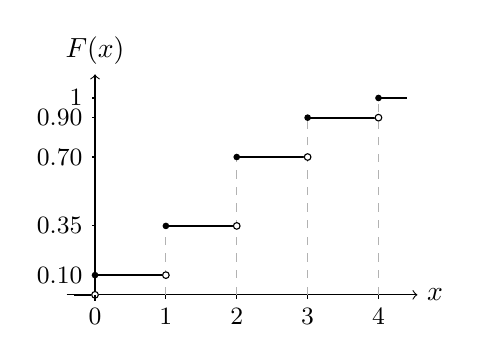
\begin{tikzpicture}[x=0.9cm,y=2.5cm]
  \draw[->] (-0.4,0) -- (4.55,0) node[right] {$x$};
  \draw[->] (0,-0.03) -- (0,1.12) node[above] {$F(x)$};

  \draw[dashed,gray!60] (1,0) -- (1,0.35);
  \draw[dashed,gray!60] (2,0) -- (2,0.70);
  \draw[dashed,gray!60] (3,0) -- (3,0.90);
  \draw[dashed,gray!60] (4,0) -- (4,1.00);

  \draw[thick] (-0.3,0) -- (0,0);
  \draw[thick] (0,0.10) -- (1,0.10);
  \draw[thick] (1,0.35) -- (2,0.35);
  \draw[thick] (2,0.70) -- (3,0.70);
  \draw[thick] (3,0.90) -- (4,0.90);
  \draw[thick] (4,1.00) -- (4.4,1.00);

  \filldraw[white] (0,0) circle (1.2pt);
  \draw (0,0) circle (1.2pt);
  \fill (0,0.10) circle (1.2pt);
  \filldraw[white] (1,0.10) circle (1.2pt);
  \draw (1,0.10) circle (1.2pt);
  \fill (1,0.35) circle (1.2pt);
  \filldraw[white] (2,0.35) circle (1.2pt);
  \draw (2,0.35) circle (1.2pt);
  \fill (2,0.70) circle (1.2pt);
  \filldraw[white] (3,0.70) circle (1.2pt);
  \draw (3,0.70) circle (1.2pt);
  \fill (3,0.90) circle (1.2pt);
  \filldraw[white] (4,0.90) circle (1.2pt);
  \draw (4,0.90) circle (1.2pt);
  \fill (4,1.00) circle (1.2pt);

  \foreach \x in {0,1,2,3,4}
    \draw (\x,0) -- (\x,-0.02) node[below] {\small \x};
  \foreach \y/\label in {0.10/0.10,0.35/0.35,0.70/0.70,0.90/0.90,1.00/1}
    \draw (0,\y) -- (-0.04,\y) node[left] {\small \label};
\end{tikzpicture}
\end{tabular}
\end{center}

\textbf{(b1)} \[
P(1<X\le 3)=P(X=2)+P(X=3)=0.35+0.20=0.55.
\]

\textbf{(b2)} \[
P(1<X\le 3)=F(3)-F(1)=0.90-0.35=0.55.
\]
\endgroup
\end{solution}

\vfill

% -------------------------------------------------------
\newpage
\AddToShipoutPictureFG*{\DrawQuestionPageTemplate}
\vspace*{\QuestionTopOffset}

\question
\begingroup
\small
\noindent Bir montaj hattında üretilen endüstriyel kontrol cihazları gün sonunda kalite kontrol istasyonunda test edilmektedir. Kalite mühendisi, bir vardiya boyunca tespit edilen kritik uygunsuzluk sayısını rassal değişken \(X\) ile göstermektedir. Amaç, sürecin ortalama hata yükünü ve bu yükün değişkenliğini incelemektir.

Test kayıtlarına göre \(X\)'in olasılık dağılımı aşağıdaki gibidir:
\[
\begin{array}{c|cccccc}
x & 0 & 1 & 2 & 3 & 4 & 5\\
\hline
P(X=x) & 0.08 & 0.17 & 0.25 & 0.22 & 0.18 & 0.10
\end{array}
\]

Buna göre:
\begin{enumerate}[nosep]
    \item[\textbf{(a)}] Beklenen değeri, yani \(E(X)\) değerini bulunuz.
    \item[\textbf{(b)}] \(E(X^2)\) değerini bulunuz.
    \item[\textbf{(c)}] Varyansı, yani \(\mathrm{Var}(X)\) değerini bulunuz.
\end{enumerate}
\endgroup

\begin{solution}
\begingroup
\small
\textbf{(a)} \[
E(X)=\sum xP(X=x)=0(0.08)+1(0.17)+2(0.25)+3(0.22)+4(0.18)+5(0.10)=2.55.
\]

\textbf{(b)} \[
E(X^2)=\sum x^2P(X=x)=1^2(0.17)+2^2(0.25)+3^2(0.22)+4^2(0.18)+5^2(0.10)=8.53.
\]

\textbf{(c)} \[
\mathrm{Var}(X)=E(X^2)-[E(X)]^2=8.53-(2.55)^2=8.53-6.5025=2.0275.
\]
\endgroup
\end{solution}

\vfill

% -------------------------------------------------------
\newpage
\AddToShipoutPictureFG*{\DrawQuestionPageTemplate}
\vspace*{\QuestionTopOffset}

\question
\begingroup
\small
\noindent Sürekli rassal değişken \(X\)'in olasılık yoğunluk fonksiyonu aşağıdaki gibi tanımlanmaktadır:

\[
f(x)=
\begin{cases}
c\,x, & 0\le x\le 1,\\[4pt]
c(2-x), & 1< x\le 2,\\[4pt]
0, & \text{aksi halde}.
\end{cases}
\]

Buna göre:
\begin{enumerate}[nosep]
    \item[\textbf{(a)}] \(f(x)\)'in bir olasılık yoğunluk fonksiyonu olabilmesi için \(c\) değerini bulunuz.
    \item[\textbf{(b)}] \(P(0.5\le X\le 1.5)\) olasılığını bulunuz.
    \item[\textbf{(c)}] \(E(X)\) değerini bulunuz.
    \item[\textbf{(d)}] \(\mathrm{Var}(X)\) değerini bulunuz.
\end{enumerate}
\endgroup

\begin{solution}
\begingroup
\small
\textbf{(a)} \[
\int_0^1 cx\,dx+\int_1^2 c(2-x)\,dx=\frac{c}{2}+\frac{c}{2}=c=1.
\]
Dolayısıyla \(\boxed{c=1}\).

\textbf{(b)} \[
P(0.5\le X\le 1.5)=\int_{0.5}^{1}x\,dx+\int_{1}^{1.5}(2-x)\,dx
=\frac{3}{8}+\frac{3}{8}=\frac{3}{4}=0.75.
\]

\textbf{(c)} \[
E(X)=\int_0^1 x(x)\,dx+\int_1^2 x(2-x)\,dx
=\int_0^1 x^2\,dx+\int_1^2 (2x-x^2)\,dx=1.
\]

\textbf{(d)} \[
E(X^2)=\int_0^1 x^2(x)\,dx+\int_1^2 x^2(2-x)\,dx
=\int_0^1 x^3\,dx+\int_1^2 (2x^2-x^3)\,dx=\frac{7}{6}.
\]
\[
\mathrm{Var}(X)=E(X^2)-[E(X)]^2=\frac{7}{6}-1=\frac{1}{6}.
\]
\endgroup
\end{solution}

\vfill

\end{questions}

\end{document}
